\subsection{改良卡鲁塞尔氧化沟}
\subsubsection{设计基本参数}
根据进出水水质(表 \ref{tab:in water})和氧化沟设计要求,将基本条件汇总如下所示:
\begin{table}[H]
	\centering
	\caption{氧化沟设计基本参数}
	\begin{tabular}{p{0.37\textwidth} *{2}{p{0.1\textwidth}}p{0.25\textwidth}}
		\toprule
		参数    & 符号    & 值     & 单位 \\
		\midrule
		设计流量  & $Q$ & 35000 & m$^3$/d \\
		综合生活污水量变化系数 & $K_z$ & 1.66 &  \\
		最低水温  & $T_{min}$  & 8     & ℃ \\
		最高水温  & $T_{max}$  & 25    & ℃ \\
		\midrule
		进水生物需氧量(BOD$_5$)浓度 & $S_0$    & 260   & mg/L \\
		进水悬浮物(SS)浓度 & $SS_0$   & 280   & mg/L \\
		进水总氮(TN)浓度 & TNK   & 45    & mg/L \\
		进水氨氮(NH$_4^+$-N)浓度 & NH$_3$-N & 35    & mg/L \\
		进水总磷(TP)浓度 & TP    & 3     & mg/L \\
		\midrule
		出水生物需氧量(BOD$_5$)浓度 & $S_e$    & 10    & mg/L \\
		出水悬浮物(SS)浓度 & $SS_e$   & 10    & mg/L \\
		出水总氮(TP)浓度 & TP    & 0.15  & mg/L \\
		出水氨氮(NH$_4^+$-N)浓度 & NH$_3$-N & 5     & mg/L \\
		出水总磷(TN)浓度 & TN    & 15    & mg/L \\
		\midrule
		污泥总产率系数 & $Y_t$ & 0.7 & kgVSS/kgBOD$_5$ \\
		混合液悬浮固体浓度(MLSS) & $X$ & 4 & g/L(MLVSS/MLSS=0.6) \\
		\makecell[l]{混合液挥发性悬浮固体浓度\\(MLVSS)} & $X_V$ & 2.4 & g/L \\
		好氧区设计污泥龄 & $\theta_c$ & 20 & d \\
		污泥自身氧化系数 & $K_d$ & 0.05 & d$^{-1}$ \\
		SS的污泥转换率 & $f$ & 0.6 & gMLSS/gSS \\
		\bottomrule
	\end{tabular}%
	\label{tab:Basic conditions for oxidation ditch design}%
\end{table}%


\subsubsection{好/缺/厌氧区计算}

\begin{figure}[H]
  \centering
  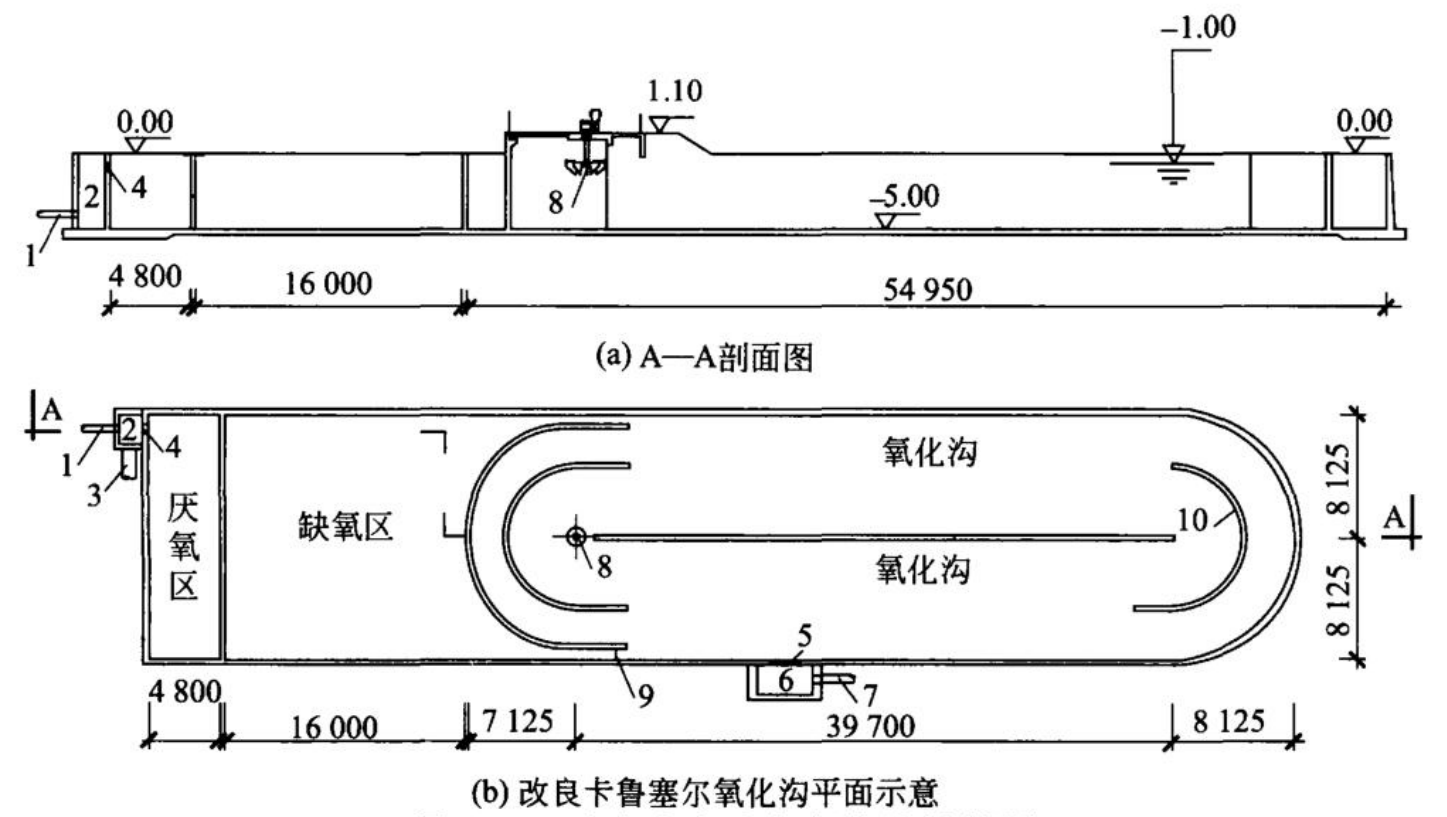
\includegraphics[width=\textwidth]{figures/Sketch of the modified Carrousel oxidation ditch.png}
  \caption{改良卡鲁塞尔氧化沟计算草图}
  \label{fig:carrousel-oxidation-ditch}
\end{figure}

\begin{enumerate}
	\item 好氧区容积 $V_1$
	\begin{align}
		V_1=\dfrac{Q(S_0-S_e)\theta_c Y_t}{1000X} &=\dfrac{35000\times(260-10)\times 20\times 0.7}{1000 \times 4} \;\text{m$^3$} \\
		&=\eval{\dfrac{35000\times(260-10)\times 20\times 0.7}{1000 \times 4}} \;\text{m$^3$} \notag
	\end{align}
	好氧区水力停留时间$t_1$为
	\begin{align}
		t_1=\dfrac{V_1}{Q}=\dfrac{30625}{35000} \;\text{d} =\eval{\dfrac{30625}{35000}} \;\text{d} =\eval{\dfrac{30625}{35000}*24} \;\text{h}
	\end{align}
	\item 缺氧区容积$V_2$缺氧区 容积采用反硝化动力学计算。
	\begin{align}
		V_2=\dfrac{0.001Q(N_k-N_{te})-0.12\Delta X_V}{K_{de}X}
		\label{eq:Volume of oxidation ditch hypoxic zone}
	\end{align}
	$V_2$——缺氧区有效容积,m$^3$;\par
	$N_k$——生物反应池进水总凯氏氮浓度,mg/L;\par
	$N_{te}$——生物反应池出水总氮浓度,mg/L;\par
	$\Delta X_V$——排出生物反应池系统的微生物量,kgMLVSS/d;\par
	$K_{de}$——脱氮速率,kgNO$_3^-$-N/(kgMLSS $\cdot$ d)。
	\begin{enumerate}
		\item 脱氮速率$K_{de(T)}$
		\begin{equation}
			K_{de(T)}=K_{de(20)}\theta^{T-20}
		\end{equation}
		$K_{de(20)}$——20℃时的脱氮速率,kgNO$_3^-$-N/(kgMLSS $\cdot$ d),取$K_{de(20)}$=0.06 kgNO$_3^-$-N/(kgMLSS $\cdot$ d);\par
		$\theta$——温度系数,取1.06;\par
		$T$——设计水温,℃,取8℃。

		所以,带入公式解得:
		\begin{align*}
			K_{de(T)}=K_{de(20)}\theta^{T-20}&=0.06\times 1.06^{8-20} \quad\text{kgNO$_3^-$-N/(kgMLSS $\cdot$ d)} \\ 
			&=0.030 \quad\text{kgNO$_3^-$-N/(kgMLSS $\cdot$ d)}
			% &=\eval{0.06\times 1.06^{8-20}}[3] \quad\text{kgNO$_3^-$-N/(kgMLSS $\cdot$ d)}
		\end{align*}

		\item 排出生物反应池系统的微生物量$\Delta X_V$
		\begin{equation}
			\Delta X_V=yY_t\dfrac{Q(S_0-S_e)}{1000}
		\end{equation}
		$Y_t$——污泥总产率系数,kgMLSS/kgBOD$_5$,取 0.7 kgMLSS/kgBOD$_5$;\par
		$y$——MLSS中MLVSS所占比例。取$y=0.6$;\par
		$S_0$——进水BOD$_5$浓度,mg/L;\par
		$S_e$——出水BOD$_5$浓度,mg/L。

		所以,带入公式解得:
		\begin{align*}
			\Delta X_V=yY_t\dfrac{Q(S_0-S_e)}{1000} &=0.6\times 0.7\times\dfrac{35000\times(260-10)}{1000} \quad\text{kgMLVSS/d} \\ 
			&=\eval{0.6\times 0.7\times\dfrac{35000\times(260-10)}{1000}} \quad\text{kgMLVSS/d} 
		\end{align*}

		\item 缺氧容积$V_2$
		
		将所求数据带入公式 \ref{eq:Volume of oxidation ditch hypoxic zone} 求解:
		\begin{align*}
			V_2=\dfrac{0.001Q(N_k-N_{te})-0.12\Delta X_V}{K_{de}X} &= \dfrac{0.001\times35000\times(45-15)-0.12\times 3675}{0.030\times 4.0} \;\text{m$^3$} \\
			&= \eval{\dfrac{0.001\times35000\times(45-15)-0.12\times 3675}{0.030\times 4.0}} \;\text{m$^3$} 
		\end{align*}
		则缺氧区水力停留时间$t_2$为
		\begin{align}
			t_2=\dfrac{V_2}{Q}=\dfrac{5075}{35000} \;\text{d} =\eval{\dfrac{5075}{35000}} \;\text{d} =\eval{\dfrac{5075}{35000}*24} \;\text{h} 
		\end{align}
	\end{enumerate}
	\item 厌氧区容积$V_3$,m$^3$
	
	取厌氧区水力停留时间$t_3=1.5$ h\footnote{《室外排水设计规范》(GB 50014-2006):厌氧区水力停留时间 $1\sim 2$ h。},则
	\begin{align*}
		V_3= Qt_3=\dfrac{35000}{24}\times 1.5 \;\text{m$^3$} =\eval{\dfrac{35000}{24}\times 1.5} \;\text{m$^3$} 
	\end{align*}

	\item 氧化沟总容积$V$及停留时间$t$
	\begin{equation}
		V=V_1+V_2+V_3 = 30625 + 5075 + 2187.5 \;\text{m$^3$} = \eval{30625 + 5075 + 2187.5} \;\text{m$^3$}
	\end{equation}
	\begin{equation}
		t=\dfrac{V}{Q}=\dfrac{37887.5}{35000} \;\text{d} = \eval{\dfrac{37887.5}{35000}} \;\text{d} = \eval{\dfrac{37887.5}{35000}*24} \;\text{h}
	\end{equation}

	\item 校核污泥负荷
	\begin{align}
		N=\dfrac{QS_0}{X_VV_1} &=\dfrac{35000\times \dfrac{260}{1000}}{2.4\times 30625} \quad\text{kgBOD$_5$/(kgMLVSS $\cdot$ d)} \\
		&=\eval{\dfrac{35000\times \dfrac{260}{1000}}{2.4\times 30625}} \quad\text{kgBOD$_5$/(kgMLVSS $\cdot$ d) (符合要求)} \notag
	\end{align}

	\item 剩余污泥量
	\begin{align} \label{eq:Amount of sludge remaining}
		\Delta X &=Y_tQ(S_0-S_e)-K_d V_1 X_V +fQ(SS_0-SS_e) \\
		&=0.7\times 35000 \times (260-10) \times 10^{-3} -0.05\times 30625 \times 4 \notag \\ 
		&\phantom{=} +0.6\times 35000\times (280-10) \times 10^{-3} \;\text{kg/d} \notag \\
		&= \eval{0.7\times 35000 \times (260-10) \times 10^{-3} -0.05\times 30625 \times 4+0.6\times 35000\times (280-10) \times 10^{-3}} \;\text{kg/d} \notag
	\end{align}
	则剩余1kgBOD$_5$产生污泥量
	\begin{align}
		\dfrac{\Delta X}{Q(S_0-S_e)} &= \dfrac{5670}{35000\times (260-10)\times 10^{-3}} \;\text{(kgDS/kgBOD$_5$)} \\
		&=\eval{\dfrac{5670}{35000\times(260-10)\times 10^{-3}}} \;\text{(kgDS/kgBOD$_5$)} \notag
	\end{align}

	\item 污⽔需氧量AOR

	因为 $a=1.47$,$b=4.57$,$c=1.42$,则
	\begin{align}
		\text{AOR} &=0.001 a Q(S_0-S_e)-c\Delta X_V +b[0.001Q(N_k-N_{ke})-0.12\Delta X_V] \\
		&\phantom{= } -0.62b\left[0.001Q(N_t-N_{ke}-N_{oe})-0.12\Delta X_V\right] \notag \\
		& = 0.001\times 1.47\times 35000\times(260-10)-1.42\times 3675  \notag \\
		& \phantom{= } +4.57\times\left[0.001\times 35000\times(45-5)- 0.12\times 3675\right] \notag \\
		&\phantom{= } -0.62\times4.57\times\left[0.001\times35000\times(45-5-10)-0.12\times 3675\right] \notag \\
		& = \eval{0.001\times 1.47\times 35000\times(260-10)-1.42\times 3675 +4.57\times\left[0.001\times 35000\times(45-5) - 0.12\times 3675\right]-0.62\times4.57\times\left[0.001\times35000\times(45-5-10)-0.12\times 3675\right]} \;\text{(kgO$_2$/d)} \notag
	\end{align}

最大需氧量与平均需氧量之比为1.58,则
\begin{align}
	\mathrm{AOR_{max}} &= 1.58 \text{AOR}=1.58 \times 10301.0894 \;\text{(kgO$_2$/d)} \\
	&= \eval{1.58 \times 10301.0894}[3] \;\text{(kgO$_2$/d)} \notag \\
	&= \eval{1.58 \times 10301.0894/24}[3] \;\text{(kgO$_2$/h)} \notag
\end{align}
\begin{align}
\text{去除1kgBOD$_5$需氧量} &= \dfrac{\mathrm{AOR_{max}}}{Q(S_0-S_e)} \\
&= \dfrac{16275.721}{35000 \times (260-10)\times 10^{-3}} \;\text{(kgO$_2$/kgBOD$_5$)} \notag \\
&=\eval{\dfrac{16275.721}{35000 \times (260-10)\times 10^{-3}}}[3] \;\text{(kgO$_2$/kgBOD$_5$)} \notag
\end{align}

	\item 氧化沟尺寸
	
	设氧化沟为2组,则单组氧化沟有效容积为
	\begin{equation}
		V_{\text{单}}=\dfrac{V}{2}=\dfrac{37887.5}{2} \;\text{m$^3$}=\eval{\dfrac{37887.5}{2}} \;\text{m$^3$}
	\end{equation}
	取氧化沟有效水深 $h=4$ m\footnote{《室外排水设计标准》(GB 50014-2021):氧化沟有效水深的确定应考虑曝气、混合、推流的设备性能,宜采用$3.5\sim 4.5$ m。},超高为 $h_0=1.0$ m\footnote{《室外排水设计标准》(GB 50014-2021):当好氧区的充氧器采用转刷、转碟时,氧化沟的设备平台高出设计水面宜为0.5 m;当采用竖轴表曝机时,宜为 $0.6 \;\text{m}\sim 0.8 \;\text{m}$,氧化沟的设备平台宜高出设计水面 $0.8 \;\text{m}\sim 1.2 \;\text{m}$。},则单组氧化沟面积为
	\begin{equation}
		A_{\text{单}}=\dfrac{V_{\text{单}}}{h}=\dfrac{18943.75}{4} \;\text{m$^2$}=\eval{\dfrac{18943.75}{4}}[2] \;\text{m$^2$}
	\end{equation}
	氧化沟高度为
	\begin{equation}
		H=h+h_0 = 4+1.0 \;\text{m} =5 \;\text{m}
	\end{equation}
	\begin{enumerate}
		\item 好氧区尺寸
		
		单组氧化沟好氧区容积
		\begin{equation}
			V_{1\text{单}}=\dfrac{V_1}{2}=\dfrac{30625}{2} \;\text{m$^3$} = \eval{\dfrac{30625}{2}} \;\text{m$^3$}
		\end{equation}
		好氧区面积
		\begin{equation}
			A_{1\text{单}}=\dfrac{V_{1\text{单}}}{h}=\dfrac{15312.5}{4} \;\text{m$^2$} = \eval{\dfrac{15312.5}{4}} \;\text{m$^2$}
		\end{equation}
		好氧区采用2沟道,单沟道宽度取 $b=8$ m,中间分隔墙厚度取 $d=0.25$ m。

		弯道部分面积(半圆)
		\begin{equation}
			A_{1\text{弯}}=2\cdot\dfrac{\pi b^2}{2} =2\times\dfrac{\pi\cdot 8^2}{2} \;\text{m$^2$} = \eval{2\times\dfrac{\pi\cdot 8^2}{2}}[2] \;\text{m$^2$}
		\end{equation}
		直线段部分面积
		\begin{equation}
			A_{1\text{直}}=A_{1\text{单}}-A_{1\text{弯}}=3828.125-200.96 \;\text{m$^2$} = \eval{3828.125-200.96} \;\text{m$^2$}
		\end{equation}
		直线部分长度
		\begin{equation}
			L_{1\text{直}} =\dfrac{A_{1\text{直}}}{2b} =\dfrac{3627.165}{2\times 8} \;\text{m} =\eval{\dfrac{3627.165}{2\times 8}}[3] \;\text{m}
		\end{equation}

		\item 缺氧区尺寸
		
		单组氧化沟缺氧区容积
		\begin{equation}
			V_{2\text{单}}=\dfrac{V_2}{2}=\dfrac{5075}{2} \;\text{m$^3$} = \eval{\dfrac{5075}{2}} \;\text{m$^3$}
		\end{equation}
		缺氧区面积
		\begin{equation}
			A_{2\text{单}}=\dfrac{V_{2\text{单}}}{h}=\dfrac{2537.5}{4} \;\text{m$^2$} = \eval{\dfrac{2537.5}{4}} \;\text{m$^2$}
		\end{equation}
		缺氧区宽度$B_2$与好氧区沟道同宽,则
		\begin{equation}
			B_2=b+d+b=8+0.25+8 \;\text{m} =16.25 \;\text{m}
		\end{equation}
		缺氧区长度
		\begin{equation}
			L_{2} =\dfrac{A_{2\text{单}}}{B_2} =\dfrac{634.375}{16.25} \;\text{m} =\eval{\dfrac{634.375}{16.25}}[3] \;\text{m}
		\end{equation}

		\item 厌氧区尺寸
		
		单组氧化沟厌氧区容积
		\begin{equation}
			V_{3\text{单}}=\dfrac{V_3}{2}=\dfrac{2187.5}{2} \;\text{m$^3$} = \eval{\dfrac{2187.5}{2}} \;\text{m$^3$}
		\end{equation}
		厌氧区面积
		\begin{equation}
			A_{3\text{单}}=\dfrac{V_{3\text{单}}}{h}=\dfrac{1093.75}{4} \;\text{m$^2$} = \eval{\dfrac{1093.75}{4}} \;\text{m$^2$}
		\end{equation}
		厌氧区长度$L_3$与好氧区沟道同宽
		\begin{equation}
			L_3=b+d+b=8+0.25+8 \;\text{m} =16.25 \;\text{m}
		\end{equation}
		厌氧区宽度
		\begin{equation}
			B_{3} =\dfrac{A_{3\text{单}}}{L_3} =\dfrac{273.4375}{16.25} \;\text{m} =\eval{\dfrac{273.4375}{16.25}}[3] \;\text{m}
		\end{equation}
	\end{enumerate}
\end{enumerate}


